\documentclass[12pt, a4paper, oneside, openright]{book}

\renewcommand{\baselinestretch}{1.24} %set line space

\setlength{\textheight}{19.8cm} %set margin size
\setlength{\oddsidemargin}{1.46cm}

\usepackage{vuwthesis} % sets up some local things, mostly the front page

\usepackage{palatino} % sets palatino as the default font
\usepackage{amsmath}
\usepackage{amssymb}
\usepackage{mathrsfs}
\usepackage{url} % for typesetting urls
\usepackage{siunitx}
\usepackage{bm}
\usepackage{graphicx}
\usepackage{caption}
\usepackage{subcaption}
\usepackage{placeins}
\usepackage{marginnote}
	\renewcommand*{\marginfont}{\color{red}\sffamily\tiny}
%\renewcommand{\baselinestretch}{1.00}


\begin{document}

\frontmatter
% Book style knows about front matter
% Report style doesn't so you need to set roman numbering etc yourself :-(

%%%%%%%%%%%%%%%%%%%%%%%%%%%%%%%%%%%%%%%%%%%%%%%%%%%%%%%

\title{Research Paper Analysing Tie Breaking}
\author{Magnus E.\ Bugge}

\subject{Data Science}
\abstract{Investigation of tie breaking and omitting Na values on differenet libraries performance. New tie breaking idea is implemented and compared with other tie breaking methods. Data used for this is pulled from previously articles in the field.}
% Books don't normally have abstracts, and this is a bit of a hack

% Uncomment the appropriate degree
%\phd
%\mscthesisonly
%\mscwithhonours
%\mscbothparts
\otherdegree{Undergraduate Research Project}



%%%%%%%%%%%%%%%%%%%%%%%%%%%%%%%%%%%%%%%%%%%%%%%%%%%%%%%




\maketitle


\tableofcontents


%%%%%%%%%%%%%%%%%%%%%%%%%%%%%%%%%%%%%%%%%%%%%%%%%%%%%%%

% book style knows about mainmatter
% if you are using report style you will have to rest page numbering etc.
\mainmatter

%%%%%%%%%%%%%%%%%%%%%%%%%%%%%%%%%%%%%%%%%%%%%%%%%%%%%%%

% individual chapters included here


\chapter{Introduction}

Time series is an important category of data since climate, finance, and health data all can be structured as time series. Classical regression, clustering and classification of time series data often works by analysing the observed values directly. Ordinal Patterns(OPs) take a different approach to time series analysis.
Instead of using the observed values, OPs transform those values into symbols.
These symbols retain information about the relative values, and aspire to capturing relevant information about the time series and the process that produced it.

Ordinal Patterns have been around for twenty years.
They were proposed by Bandt and Pompe in 2002~\cite{Bandt2002}.
This seminal article has received, to date, over \num{3000} citations on the Web of Science.
Their main properties are invariance, robustness, and being model-agnostic.

OPs have been used in applications in several domains.
Many of these applications involve comparing time series, signals, and images through features extracted from their Ordinal Patterns.
Since results about the distribution of such features are recent, our initial interest was comparing existing conclusions with those supported by the new statistical tests.
While approaching this research avenue, we found indications of reproducibility crisis~\cite{Fidler2018} in this field, mostly related to data availability.
We then moved into the application of these new tests to already published results, and found evidence of the other type of reproducibility crisis: diverging results depending on the type of library employed.
We decided to study the effect of preprocessing of the data by a combination of omitting Na values and adding noise to break ties. A new tie breaking method is proposed and its performance on computing entropy and p values is investigated.

We are interested in verifying the reproducibility of results of Ordinal Patterns in the scientific literature.
Initially, we wanted to check how many of the 3000 articles, were reproducible. This was a big task, so at first it was narrowed down to just papers focusing on climate. In the end, around 31 papers were investigated deeply.

\chapter{Ordinal Patterns}

\section{History}
Bandt and Pompe's first paper about ordinal patterns is from 2002. 
They introduced the concept of turning a time series or signal into a sequence of symbols. 
They furthermore used the Shannon entropy on the symbol distribution~\cite{Bandt2002}. 
The Shannon Entropy was developed in 1948 by C.\ E.\ Shannon~\cite{Shannon1948} as a way to quantify uncertainty and unpredictability.

The 1995 paper ``A statistical measure of complexity'' by López-Ruiz et al.~\cite{LopezRuiz1995} introduced the concept of a statistical measure of complexity. 
This idea was applied to OPs in 2003~\cite{Martin2003}, and in 2004 the version of it using Jensen-Shannon divergence was published~\cite{Lamberti2004}.
We use the latter in this work.

\section{Definition}

Every analysis that employs OPs starts by defining the (integer-valued) word size $D\in\{2,3,\dots\}$ and time lag $\tau$.
We will only use $\tau=1$, and thus will drop, it from the following discussion.

Consider the finite time series of real values $\bm x=(x_1, x_2,\dots, x_{n+D-1})$. 
The word size $D$ is chosen, as seen in the bibliometric analysis below, a word size between 3-6 is most common.
The Bandt \& Pompe transformation (also called ``BP Symbolisation'') converts each subset of size $D$ of contiguous and different values into a symbol, i.e.,
the first tuple of $D$ values will be $(x_1,x_2,\dots,x_{D})$, 
the second tuple will be $(x_2, x_3,\dots,x_{D+1})$, and so on.

There are at least two ways of computing OPs.
We will describe one of them.
Each tuple is transformed into a pattern by ranking them by numerical order. 
The lowest observation gets assigned the number $0$ and the highest observation gets the number $D-1$. 
The pattern can then be written as a string of these numbers. 
The tuple $(0.51, 0.79, 0.14)$ will have pattern $1,2,0$.
How we write the patterns is transparent, provided there is only one pattern for each possible sorting of the tuple.
For example, we could have defined that $(0.51, 0.79, 0.14)$ becomes $\pi^3$ or $c$ or $\mathfrak{c}$.
Assuming there are no ties in each word, there are $D!$ possible patterns that we will denote $\bm\Pi=\{\pi^1,\pi^2,\dots,\pi^{D!}\}$.

By applying the BP symbolisation, we transform the time series 
$\bm x = (x_1, x_2, \dots, x_{n+D-1})$ into the sequence of symbols
$\bm \pi = (\pi_1, \pi_2,\dots, \pi_n)$.
The observed frequency pattern $\widehat{p}_i$ is defined as,
$$
\widehat{p}_i=\frac{\#\{t : \pi_t = \pi^i\}}{n} ,
$$
with which we define the vector of observed proportions:
$$
\widehat{\bm p} = (\widehat{p}_1, \widehat{p}_2, \dots, \widehat{p}_{D!}).
$$



A tie is when a tuple contains identical values. In practice, there may be ties, for instance when observing times series registered with finite precision.
There are several ways to handle ties.
They can be ignored, i.e., no pattern is computed for tuples with ties,
or they can be broken by adding small random perturbations. 
Techniques that handle ties are usually referred to as ``imputation solutions.''

OPs are usually considered useful for time series of at least length $n>100D$.

\begin{figure}
    \centering
    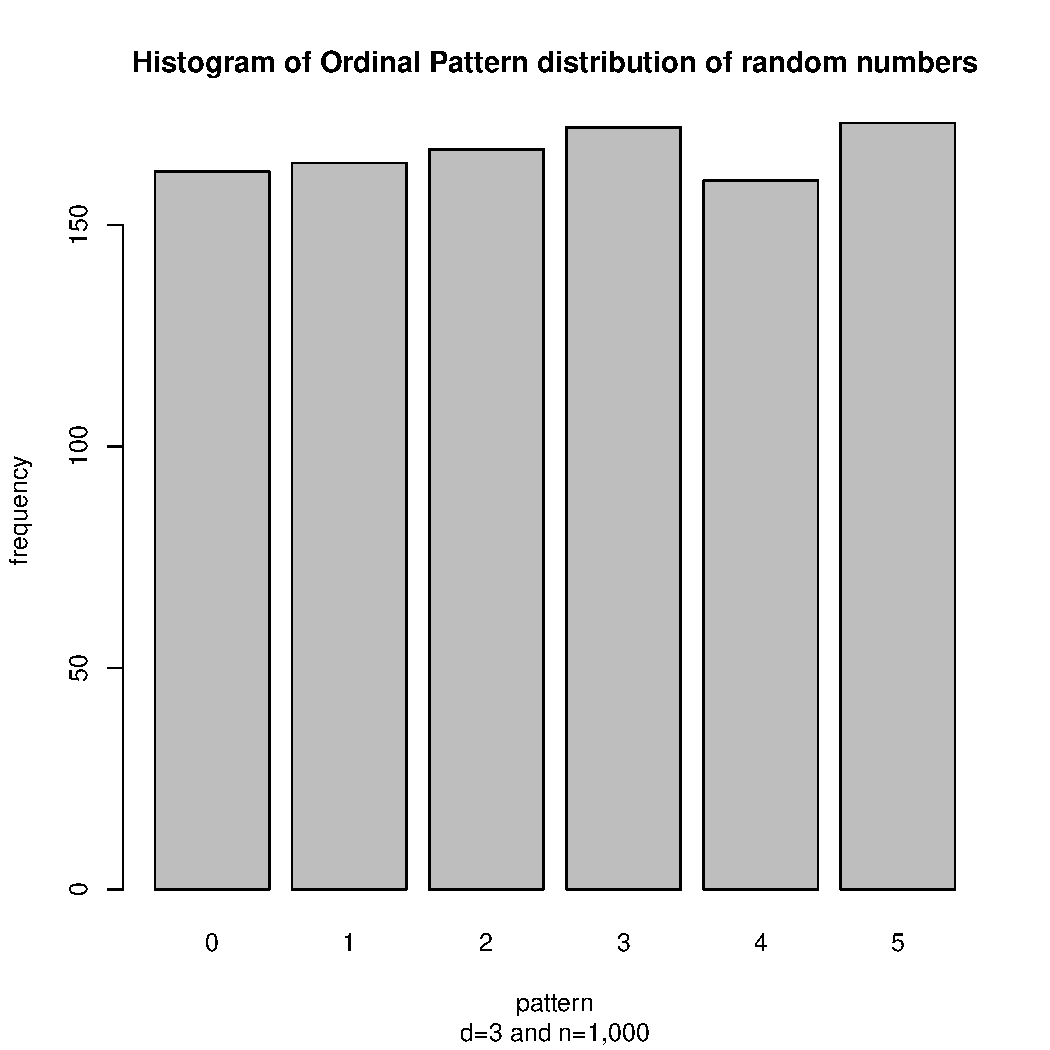
\includegraphics[width=\textwidth,keepaspectratio]{./powerlaw/histogram.pdf}
    \caption{Simple histogram of the ordinal pattern distribution of random numbers}
\end{figure}

From the ordinal pattern distribution, features can be extracted. The two main used features in this field are Entropy and Complexity. In this paper, Shannon Entropy will be used, which is defined as.

$$h(n)=-\sum p(\pi) \ln(p(\pi))$$
Normalized version
$$H(n)=-\frac{\sum p(\pi) \ln(p(\pi))}{\ln(D!)}$$

There are several statistical complexity measures that can be used. They are all a product between the used entropy and a distance measure. In this paper Martin-Plastino-Rosso intensive Statistical Complexity Measure is used, where the distance measure is Jensen-Shannon divergence, and it is measured between the pattern distribution and the uniform distribution. The $Q_0$ is normalizing term. It is defined as

$$C[\mathscr{P}]=H[\mathscr{P}]\cdot Q_J[\mathscr{P},\mathscr{P}_e]$$

$$Q_J[\mathscr{P},\mathscr{P}_e]=Q_0\cdot \mathscr{J}[\mathscr{P},\mathscr{P}_e]$$

$$\mathscr{J}[\mathscr{P},\mathscr{P}_e]=S[\frac{\mathscr{P}+\mathscr{P}_ee}{2}]-S[\frac{\mathscr{P}}{2}]-S[\frac{\mathscr{P}_e}{2}]$$

$$\mathscr{P}_e=\{p_j=\frac{1}{W};j=1...,W\}$$
$$Q_0 = -2(\frac{W+1}{W}ln(W+1)-2ln(2W)+ln(W))^{-1}$$
\cite{Amigo2023b}

\paragraph{Applications}
Going to the original Bandt and Pompe paper~\cite{Bandt2002} on Semantic Scholar and getting the ten most recent citations, gives a good picture of how broadly this methodology is being used.

The topic varies from: "Walnut crack detection..."~\cite{Zhang2024}, Schizophrenia~\cite{Wang2024}, Analysis of Smart Drilling~\cite{Szwajka2024}, Epileptic Seizure detection~\cite{AbhishekParikh2024}, mind wandering during video-based learning~\cite{Tang2024} and Random Numbers generated based on dual-channel chaotic light~\cite{Liu2024}. The rest that was found~\cite{Demirel2024, Du2024, Sun2024, Li2024}

\section{Reproducibility}
\paragraph{Reproducibility crisis}
Data from many scientific fields are analysed in data science, as shown in the application section of ordinal patterns above. It therefore increases the difficulty of reproducing the data collection stage, as most cases require an interdisciplinary study involving multiple people. In some cases, it is impossible e.g. if the equipment needed is unavailable or a time series of weather data cannot be recollected, since it is impossible to go back in time. The point of science is to eliminate trust when sharing knowledge, however, the above observations highlight the need for some degree of confidence, in cases, where data cannot be reproduced. Only data that is random numbers, generated in a script, will be reproduced in this paper.

The COVID-19 pandemic gave birth to the following quote. "We warn against the potential misuse or misleading interpretation of public data of variable quality"~\cite{Struelens2021}. Data from different governments does not have the same quality. This necessitates good source criticism. In this paper, data from peer-reviewed studies will be trusted, which have often either produced the data themselves or got it from reputable organizations such as NASA or NOAA. 

In this paper, the focus will be on direct computational reproduction.

"Computational reproducibility is most often direct (reproducing particular analysis outcomes from the same data set using the same code and software), but it can also be conceptual (analysing the same raw data set with alternative approaches, different models or statistical frameworks)"~\cite{Fidler2018}

\section{Bibliometric analysis}
31 articles were analysed for data availability and used word size. The majority of them are about climate, and they explicit have to used Permutation Entropy. Four categories were made for data availability: “Available”, “Sourced”, “On-Request” and “not Available”. Sourced is the broadest category. Some articles give a detailed description of how to pull the data from a website. Other articles give no description, except, which organisation they got the data from. The is no differentiation between these cases in the category S. A is the best category and only used, when the data is directly downloadable. R is when the dataset has to be requested by the author and is suboptimal. N is the worst category, because there is no source to data, nor is the dataset attached to the paper in any way. Word size between 2-7 were used. Some articles used multiple word sizes, which is why the sum of “No. articles using” is higher than 31. Only 4 articles data were readily downloadable. The data is definitely possible to get from some articles in category "S", but many of them were very sparse in their description of the data, to the point, where it would be hard to pull it from the website. Assuming that around half of the data from articles in "S" can be pulled from their sources. That leaves around 50\% of the article, where it is not possible to reproduce the data processing part of the article. Ideally, all papers should be reproducible and especially their data processing part, since modern technology allows for extremely efficient data sharing across vast distance to a very affordable price. According to this paper~\cite{Baker2016} more than 70\% of researches have failed reproducing an article and 52\% agree that there is significant reproducibility crisis. In this paper, cases occurred, where the data had been downloaded and verified to being true, but the data processing could not be reproduced. See figures 2.2 and 2.3. Article, which were tried to be reproduced~\cite{Saco2010}


\begin{table}[]
\begin{tabular}{|l|l|l|l|l|l|l|l|}
\hline
Word size & 2 & 3  & 4  & 5 & 6 & 7 & Multiple \\ \hline
No. articles using  & 4 & 13 & 15 & 9 & 6 & 1 & 9        \\ \hline
\end{tabular}
\end{table}

\begin{table}[]
\begin{tabular}{|l|l|l|l|}
\hline
A & S  & R & N \\ \hline
4 & 19 & 3 & 4 \\ \hline
\end{tabular}
\end{table}

\begin{figure}
    \centering
    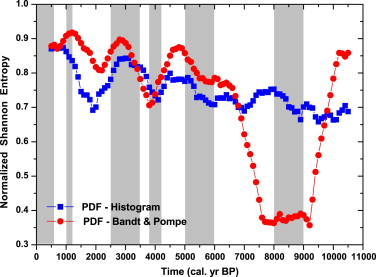
\includegraphics[width=\textwidth,keepaspectratio]{ElNino/ArticleEntropyPlot.jpg}
    \caption{Original papers entropy plot, Red dots should be equal to the dots in plots below}
\end{figure}

\begin{figure}
    \centering
    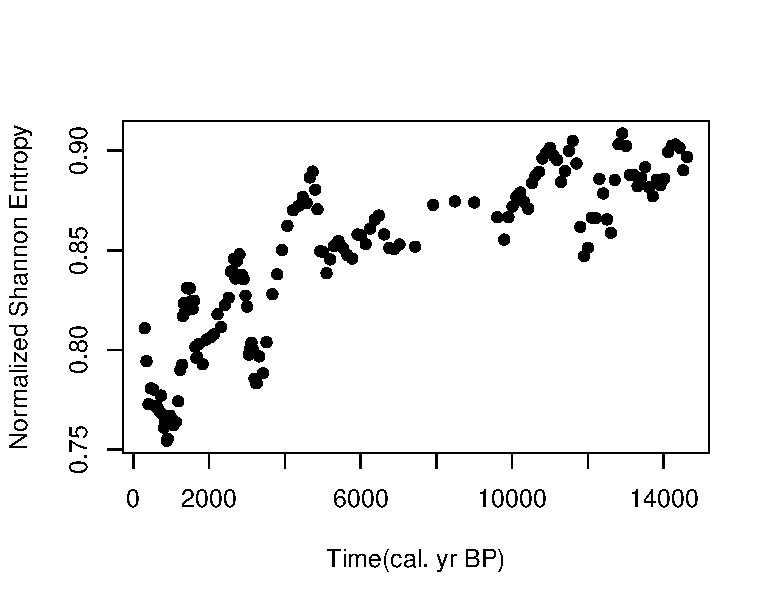
\includegraphics[width=\textwidth,keepaspectratio]{ElNino/Entropy.pdf}
    \caption{This papers reproduction. The x-axis is slightly bigger, however the data in range 0-11,000 cal. yr BP, were verified to be identical, and that is not identical in any way.}
\end{figure}
\chapter{Comparison of two time series}
\paragraph{Examples of how comparisons are done in the literature}
Ordinal Patterns have been used in astrophysics to analyse geomagnetic auroras. Two articles where found to do this. They both compare the plotted points in the HxC plane to fractional Brownian motion time series. "Many of the points are on or very near the fractional Brownian motion curve, but a single point from the Helios data lies above the fractional Brownian motion curve." \cite{Weygand2019}. A small amount of calculation is done in this paper to rate the statistical likelihood of a point being displaced from the fractional Brownian motion(fBm), but no method is presented to evaluate, if a point is displaced. "Figure 4 indicates that complexity-entropy values of AL overlap the fBm values for all subsampling parameters $\tau$" \cite{Osmane2019}. Same problem in this article, wherre no method is presented to systemic rate if a point is overlapping or not with fBm values. Ordinal patterns is often used in climate research to detect changes in the dynamics of a weather system over time. This is done in this paper \cite{Saco2010}, by splitting the dataset into windows and calculating the entropy for each window. No method is presented to evaluate if a change in entropy is significant. It is assumed that a change in entropy means a change in the dynamics of the system, without considering the possibility that it might be caused by stochastic randomness of sampling. 

\paragraph{Statistical Test and Confidence Intervals}
Confidence intervals describes the range within a sampling of a distribution has a certain percentage of being in. Statistical Test can be used to reject a wide range of hypothesises. P value is used as rejection criteria, where the lower the p values is the lower is the chance of making a type 1 error, which is rejecting a true hypothesis.\cite{Smithson2003}

\paragraph{Confidence Interval of an Ordinal Pattern Distribution Entropy}
By assuming that $\textbf{X}_n = (X_{1,n},X_{2,n},...,X_{K,n})$ with $n \in \mathbb{N}$ is a sequence of independent and identically distributed K-variate vectors of random variables. Furthermore assuming as $n$ tends to infinity, $$\sqrt{n}(X_{1,n}-\theta_1,X_{2,n}-\theta_2,...,X_{K,n}-\theta_K)$$ 
converges in distribution to the multivariate normal law $\mathscr{N}(\textbf{0},S_{\textbf{X}})$, where $S_{\textbf{X}}$ is the covariance matrix. The following terms are defined:
m is the embedding dimension.
$\mathbf{q}=(q_1,q_2,...,q_{m!})$, where $q_i$ is the probability of observing the ordinal pattern $\pi_i$.
$\mathbf{D_q}=Diag(q_1,q_2,...,q_{m!})$ Diagonal matrix.
$\mathbf{Q}^{(\ell)}$, which is the transition matrix with elements
$q_{ij}^{(\ell)}=Pr(\psi =\pi_i \wedge \psi_{t+\ell}=\pi_j)$
for $\ell = 1,2,...,m-1$


From this starting point it is derived that 
$$\sqrt{n}[S(\hat{\textbf{q}})-S(\textbf{q})] \overset{\mathscr{D}}{\underset{n\rightarrow\infty}{\longrightarrow}}\mathscr{N}(0,\sigma_{\textbf{q}}^2)$$
$$ \sigma_{\textbf{q}}^2=\sum_{i=1}^{m!}(\mathbf{\Sigma_q})_{ii}+2\sum_{i=1}^{m!-1}\sum_{j=i+1}^{m!}(\bm{\Sigma_q)}_{ij}$$

\begin{displaymath}
  (\mathbf{\Sigma_q})_{ij} = \left\{
    \begin{array}{lr}
      (ln(q_i)+1)^2\mathbf{\Sigma}_{ii} & \text{if $i=j$}\\
      (ln(q_i)+1)(ln(q_j)+1)\mathbf{\Sigma}_{ij} & \text{if $i \neq j$}
    \end{array}
  \right.
\end{displaymath} 

$$\mathbf{\Sigma}=\mathbf{D_q}-(2m-1)\mathbf{qq}^T+\Sigma_{\ell=1}^{m-1}(\mathbf{Q}^{(\ell)}+{\mathbf{Q}^{(\ell)}}^T)$$  
\cite{Rey2023}It is the variance that is of interest, as it will be used for statistical tests. The test goes as follows. Let $x=(x_1,x_2,...,x_{n_x})$ and $y=(y_1,y_2,...,y_{n_y})$ be two independent time series of length $n_x=T_x+D_x-1$ and $n_y=T_y+D_y-1$. $p_x$ and $p_y$ is the ordinal distributions of the time series. $H(\hat{p}_x)$ and $H(\hat{p}_y)$ is their entropies. A new distribution W is constructed. $W \overset{D}{\rightarrow}\mathscr{N}(\mu_W,\sigma_W^2)$, with $\mu_W=\mu_{n_x,p_x}-\mu_{n_y,p_y}$ and $\sigma_W^2=\sigma_{n_x,p_x}^2+\sigma_{n_y,p_y}^2$. 
The p value ends up being $2(1-\Phi(\xi))$, where $\xi = \frac{H(\hat{p}_x)-H(\hat{p}_u)}{\sigma_W}$. \cite{Chagas2022}

\paragraph{Implementation}
The three main libraries that will be used specific to the field of ordinal patterns are: statcomp\cite{statcomp}, pdc\cite{pdc} and StatOrdPattHxC, which is a library developed by the supervisor of this project. Slight modifications are made to StatOrdPattHxC. As will be shown later these three libraries perform quite differently in a lot of cases. Solutions for this is proposed. StatOrdPattHxC has the variance and statistical test implemented, which statcomp and pdc do not. A wide range of standard R libraries is utilized as well.
\chapter{Applications}
\section{Power-law noise}

We applied the statistical test mentioned in the previous chapter on computer-generated power-law noise series.

A collection of independent and identically distributed observations from a continuous random variable is usually referred to as ``white noise.''
Its power spectrum is constant.
Other types of noise can be obtained stipulating different shapes of the power spectrum.
One of the most common ways to achieve this is by imposing spectra of the form $1/f^k$, where $f$ if the frequency and $k$ is a constant.
The case $k=0$ reverts to white noise;
if $k=1$ one has pink noise;
if $k=2$ one has Brownian noise, also called ``red noise;''
if $k=10\log_{10}2\approx 3.01$ per octave one has blue noise;
if $k=20\log_{10}2\approx 6.02$ per octave one has violet noise.
The Wikipedia page ``Colors of Noise'' available at \url{https://en.wikipedia.org/wiki/Colors_of_noise} discusses other types of noise, where they are used, and how they are called.
Timmer and König~\cite{Timmer1995} discussed ways of simulating $1/f^k$ noise.

Our study forms $k$ by choosing
$k_1\in\{1,3,5\}$, and for each $k_1$ value, we defined $k$ as $k=(k_1-e^0,k_1-e^{-1},k_1-e^{-2},k_1-e^{-3},k_1,k_1+e^{-1},k_1+e^{-2},k_1+e^{-3})$. 
The statistical test is used on every possible pair of a value from $k_1$ and each of its generated $k$ values, using series of \num{1000} observations. 
The hypothesis is rejected if the $p$-value is less than $0.05$, and we iterated ten times for each pair. 

Fig.~\ref{fig:PowerLawTests} shows the rejection rate for each $k_1$. 
The last plot shows the proportion of NaNs produced by the tests.
Power-law series with $k=5$ have entropy around $0.4$, the rest of the time series that will be examined in the paper have entropy above $0.9$, so this should not be a problem. 
The Rejection plot for $k_1=1$ is quite surprising in the sense that many values around $k_1$ have high rejection rate. 
The case $k_1=3$ corroborates that the further away a point gets from $k_1$, the larger is the rejection rate.

\begin{figure}[hbt]
    \centering
    \begin{subfigure}[b]{0.3\textwidth}
        \centering
        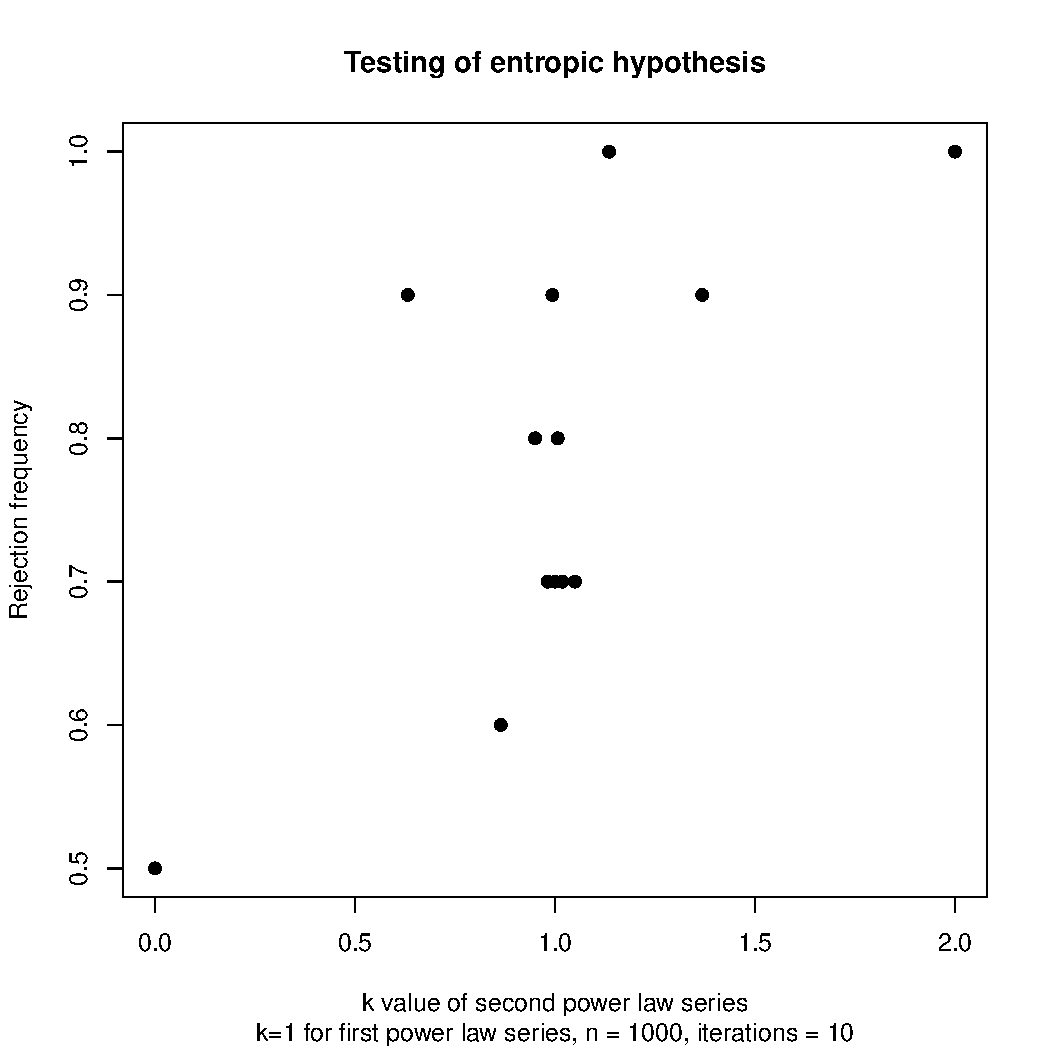
\includegraphics[height=7cm,keepaspectratio]{./powerlaw/rejectionPlot,k1=1,n=1000,iterations=10.pdf}
        % This plot was produced with lines XXX of file YYY; increase the legend size, use serif fonts
    \end{subfigure}
    \hfill
    \begin{subfigure}[b]{0.5\textwidth}
        \centering
        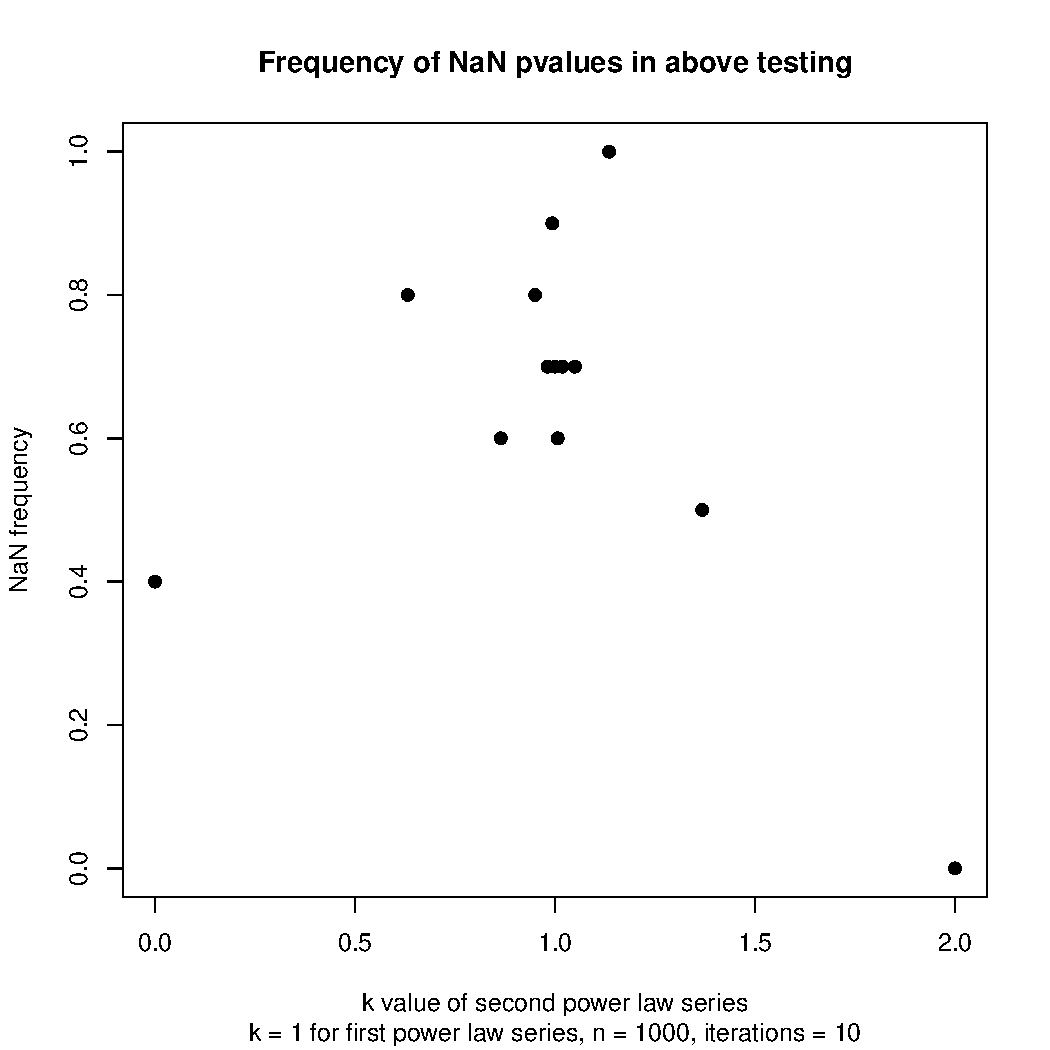
\includegraphics[height=7cm,keepaspectratio]{./powerlaw/NaNPlot,k1=1,n=1000,iterations=10.pdf}
    \end{subfigure}
    \vfill
    \begin{subfigure}[b]{0.3\textwidth}
        \centering
        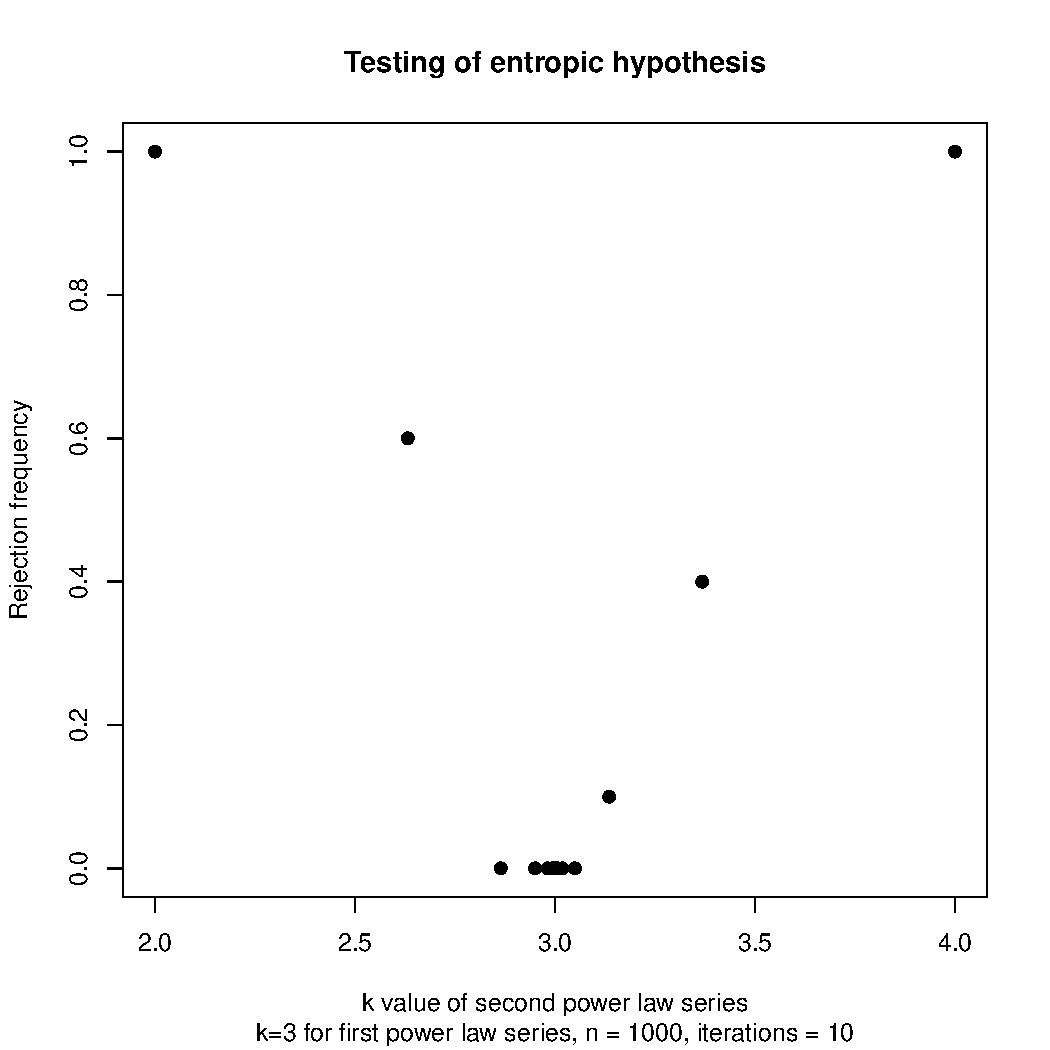
\includegraphics[height=7cm,keepaspectratio]{./powerlaw/rejectionPlot,k1=3,n=1000,iterations=10.pdf}
    \end{subfigure}
    \hfill
    \begin{subfigure}[b]{0.5\textwidth}
        \centering
        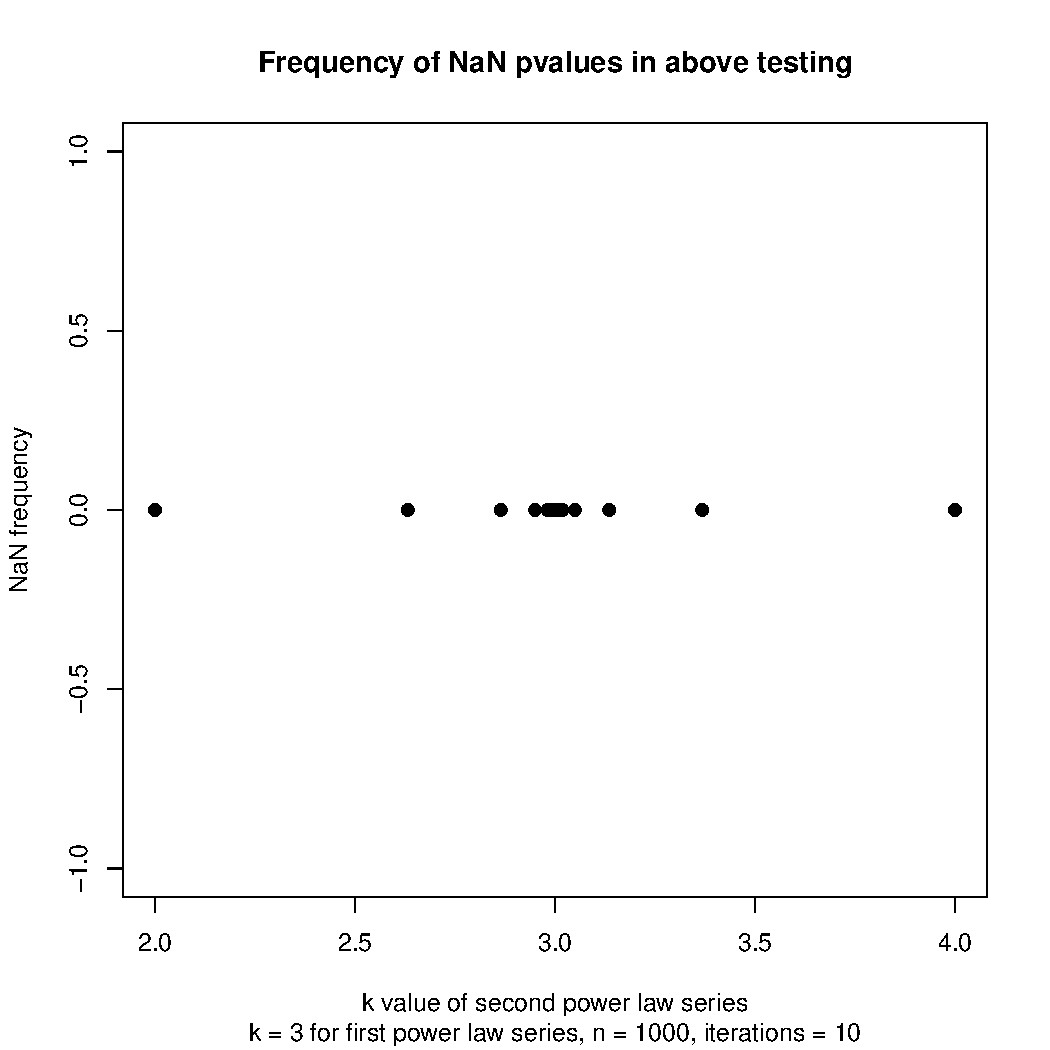
\includegraphics[height=7cm,keepaspectratio]{./powerlaw/NaNPlot,k1=3,n=1000,iterations=10.pdf}
    \end{subfigure}
    \vfill
    \begin{subfigure}[b]{0.3\textwidth}
        \centering
        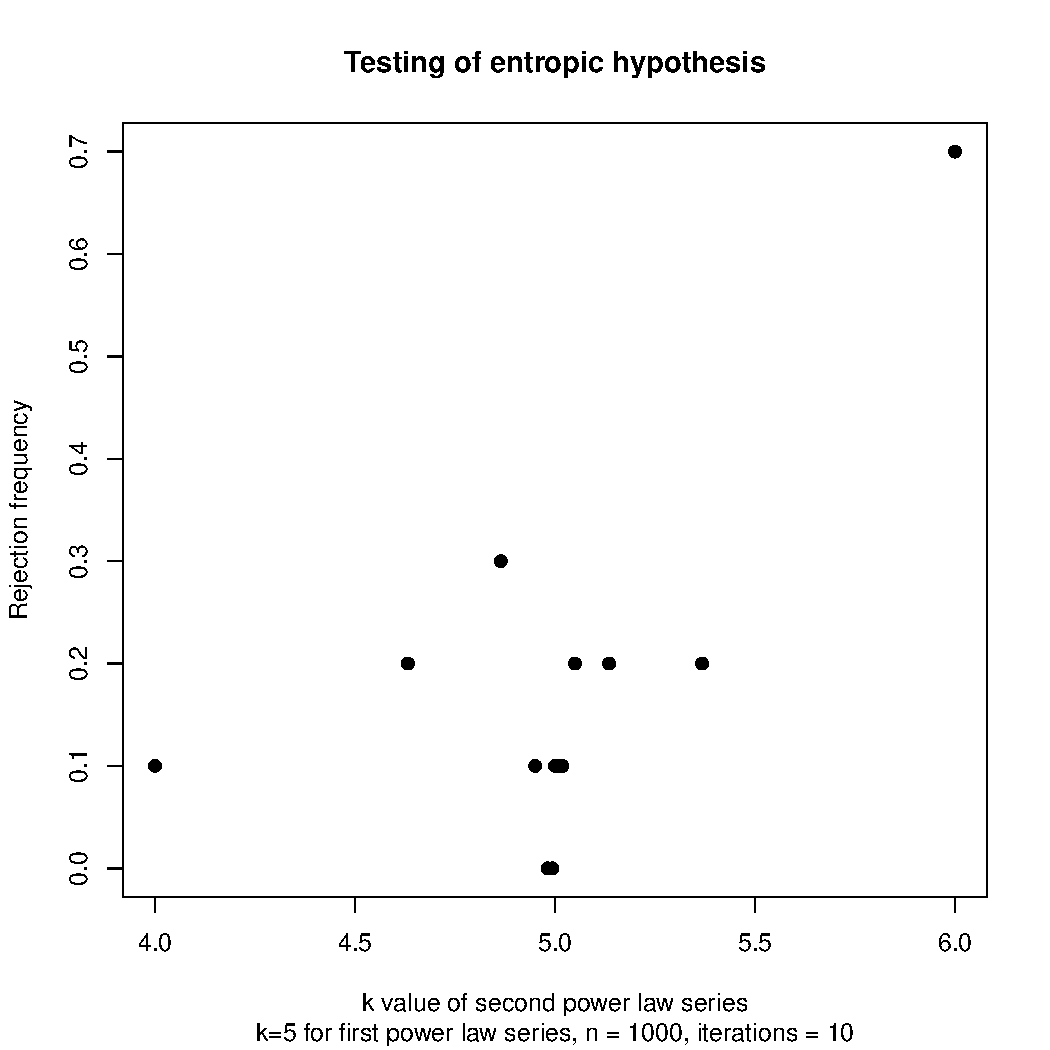
\includegraphics[height=7cm,keepaspectratio]{./powerlaw/rejectionPlot,k1=5,n=1000,iterations=10.pdf}
    \end{subfigure}
    \hfill
    \begin{subfigure}[b]{0.5\textwidth}
        \centering
        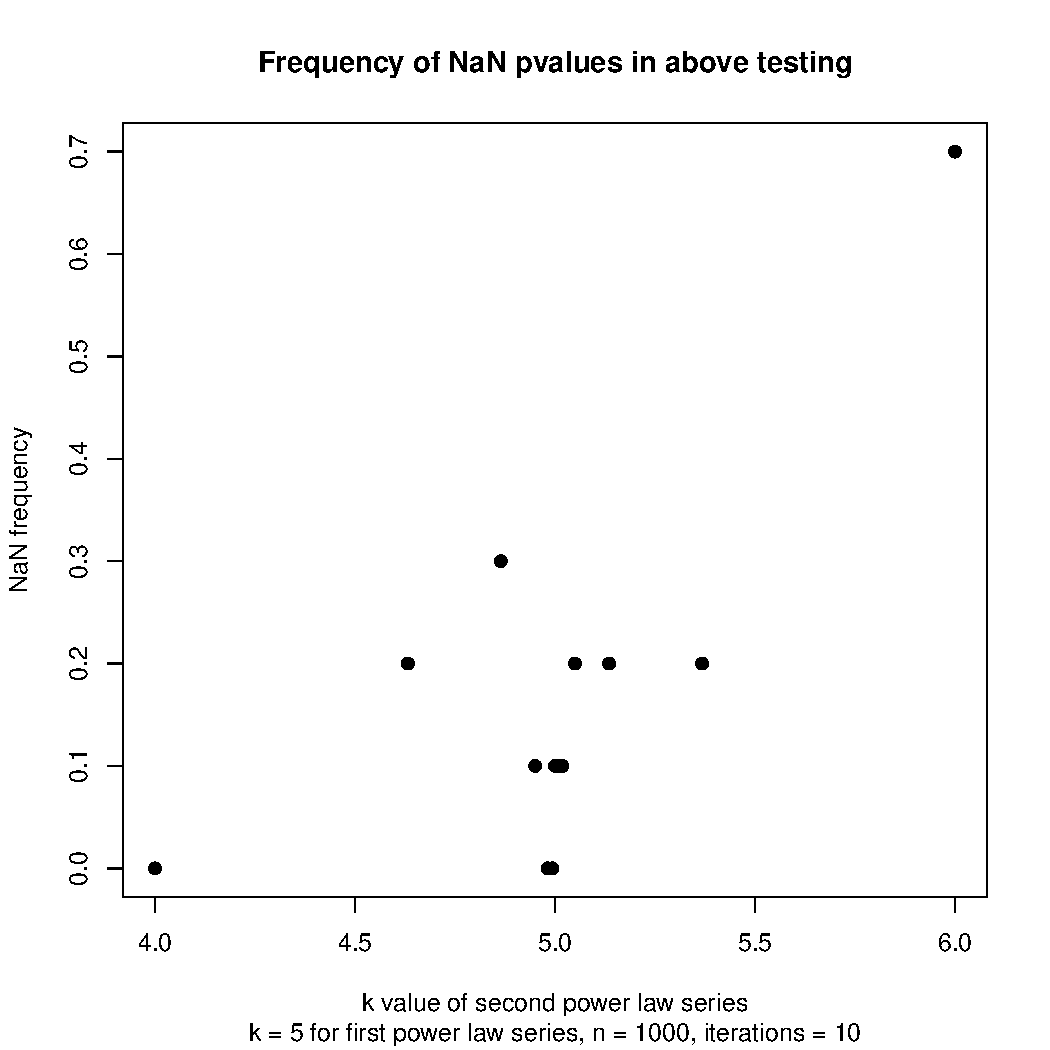
\includegraphics[height=7cm,keepaspectratio]{./powerlaw/NaNPlot,k1=5,n=1000,iterations=10.pdf}
    \end{subfigure}
    \caption{Power-law experiment}\label{fig:PowerLawTests}
\end{figure}

\FloatBarrier

\section{Idea behind new tie breaking}
In the next section, a new way to break ties will be implemented and used. The idea behind it is when having a tie, instead of either randomly assigning it to any of the possible patterns, which was proposed by Bandt and Pompe in their original paper~\cite{Bandt2002}, or always assigning a type of tie to a given pattern, which is done in the article being used in the next section~\cite{Chagas2022}, the new idea is to assign an equally large weight to all the possible patterns in case of a tie. In a tie, with k possible patterns, each of these k patterns gets a weight of $\frac{1}{k}$. The amount of possible patterns is the product of the occurrence of each unique value. To calculate the ordinal pattern distribution, simply sum up all the weights for each pattern and divide by the total amount of weight to get the frequency. Ordinal patterns are often used in fields that do science on real-world phenomena. In cases where the measuring equipment has a low precision, ties will often occur, e.g. a weight measurement. It is commonly known that objects have an atomic weight, since all everyday objects are made of particles that have an atomic weight. The atomic weight unit is $1\mu = 1.66..\cdot10^{-27}kg$, so the theoretical weight of an object has a lot of decimals, which could theoretically be measured, however putting a person on a normal household scale will only give a result in kilograms with one decimal. A person measuring themselves on a scale at different times and weighing the same does not mean they had the same atomic weight at both times. Their data would result in a tie, but based on the above argumentation it is fair to assume that in reality, the weight has either gone up or down, however, it is impossible with the given instruments to measure, which it is, so the only fair assumption is that both cases are equally likely. This can almost be seen as superposition\cite{Schroedinger1926} of the change of weight. The weight has gone both up and down until a more precise measurement is made, but until that, it is only fair to think both cases are possible and in this case equally possible. This type of tie-breaking should work, where it can be argued that a theoretical measurement has a higher precision than the actual measurement. It does, however, not make sense to use it, when the measured value can be argued to be of the same precision as a theoretical measurement, e.g. “How many cows are in front of me at a certain type?”. This implementation will briefly be referenced as “My implementation”, but mostly as a “Theoretical Split”. Note that the theoretical split method does not need noise added. Adding noise almost always removes all ties, which means it should perform identically to “article implementation”, which is the implementation made in the article\cite{Chagas2022}, since it is built upon that code. The theoretical split and the second tie-breaking solution are deterministic, whereas the Bandt and Pompe solution is stochastic.

\FloatBarrier

\section{Temperature Data}
\cite{Chagas2022} Will be partly reproduced and additional plots and tables will be made. Only the maximum temperature part of the climate data in section 6 of the article will be used. As can be seen in Figure 4.2 the percentage of ties in this dataset is extremely high. It is therefore quite important, how ties are handled since they make up a bulk of the dataset. 
\begin{figure}
    \centering
    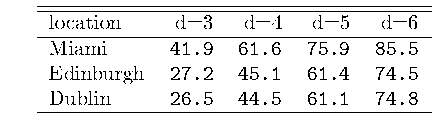
\includegraphics{./Weather/tiesTable.pdf}
    \caption{Table of ties in percentage}
\end{figure}


The libraries mentioned earlier all handle ties differently, as seen in Figure 4.3. The first three columns are the setting of each experiment. The start date column is included, because the paper, where the data is from, accidentally started their data on 1992-08-14, instead of 1992-08-08 as they said the data started from, it does however not make a big difference, which can be seen between the top three rows and bottom three rows.  If all the values in a row are identically, that means the libraries perform identically. The only setting, where this happens, is when noise is added and Na values are omitted. Na omit removes Na values and the dataset is pushed together, where the Na values have been removed. In the rest of the experiment, this setting will be used. 

\begin{figure}
    \centering
    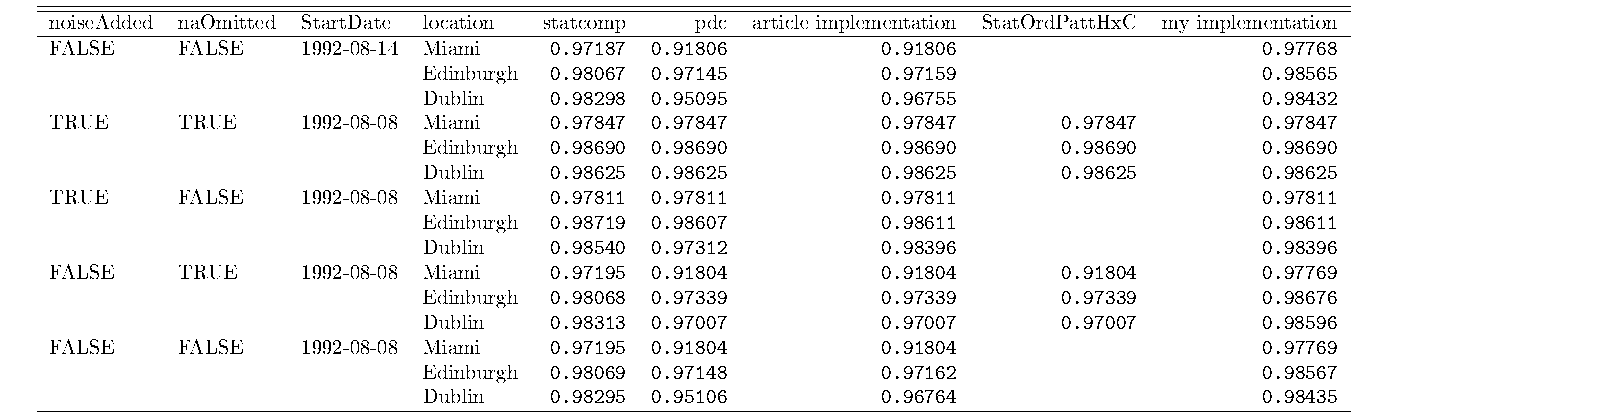
\includegraphics[width=\textwidth,keepaspectratio]{./Weather/entropyTable.pdf}
    \caption{Entropy table of libraries performs on different preprocessing}
\end{figure}

A more in-depth analysis of the Theoretical Split versus adding noise is made. The statcomp library is the comparison library, but it does not matter, which library is chosen, since they perform identically in this case. As can be seen in Figure 4.5 the theoretical value is very close to both the mean and median of the entropy of 1,000 iterations. Figure 4.4 clearly shows the problem of adding a random sample of white noise, since the values are distributed in an interval of range size around 0.003-0.004. The theoretical value is very precise, when comparing both with the median and mean of the 1,000 iterations of noise.

\begin{figure}
    \centering
    
\includegraphics[width=\textwidth,keepaspectratio]{./Weather/noiseStochasticTheoretical.pdf}
    \caption{Iterations of adding noise vs theoretical split in sorted order, the vertical line is median and horizontal is theoretical split value.}
\end{figure}

\begin{figure}
    \centering
    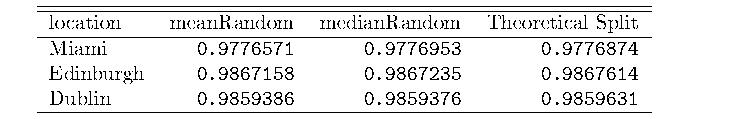
\includegraphics[width=\textwidth,keepaspectratio]{./Weather/random_vs_theoreticalSplit.pdf}
    \caption{Table of mean and median of adding noise and theoretical split. Temperature dataset}
\end{figure}

The above experiment is repeated, but where the theoretical split is fed a constant dataset. The constant values here represent very imprecise measurements, where the true values of the observed phenomenon are assumed to be different. E.g. trying to measure white noise, with a bad instrument. It is important to note that if a dataset contains just a single constant value, where the measurement is precise. The entropy would naturally be 0, since there is full predictability, e.g. “how many cows are on the field at a given time”. The iterations are calculated on random numbers, which ideally should be white noise. Figure 4.6 rarely has the entropy of ideal white noise, which is 1, where the theoretical split can correctly calculate that the poorly measured white noise has entropy 1. Figure 4.7 shows that the median measurement is closer than the mean to the theoretical split, so it might be a better measurement. In Figure 4.5 the median is generally also closer to the theoretical split. 

\begin{figure}
    \centering
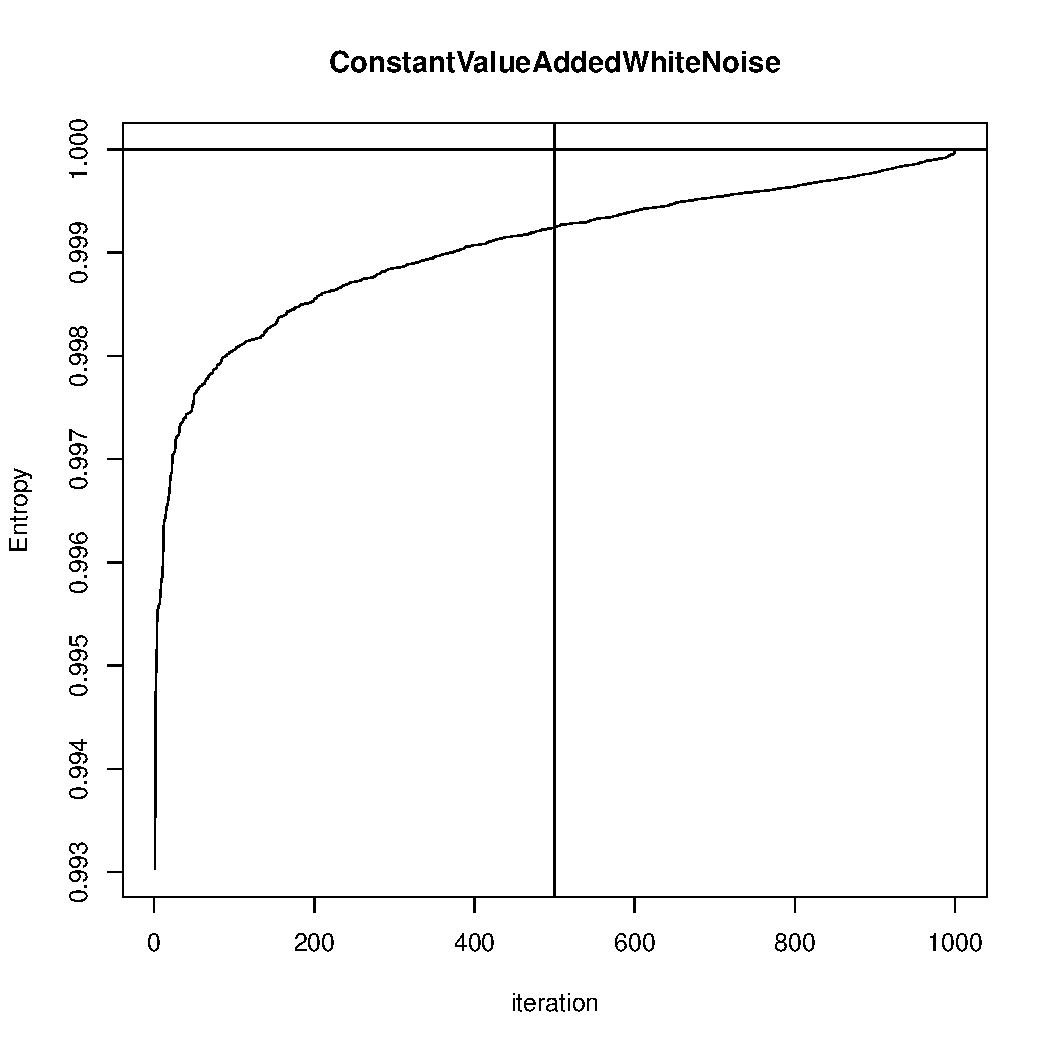
\includegraphics[width=\textwidth,keepaspectratio]{./Weather/constantWithWhiteNoiseStochasticTheoretical.pdf}
    \caption{Constant dataset}
\end{figure}

\begin{figure}
    \centering
    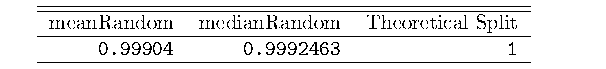
\includegraphics[width=\textwidth,keepaspectratio]{./Weather/random_vs_theoreticalSplitWhiteNoise.pdf}
    \caption{Mean and median of adding noise and theoretical split, constant dataset.}
\end{figure}

Figure 4.8 is a plot of the theoretical split values as the entropy of the three locations on the HxC plane, with confidence intervals on the entropy. At first glance, it looks like the confidence interval sticks out of the boundaries, however it is important to remember that a change in entropy leads to a change in complexity, so the confidence intervals are not breaking the boundaries, since it is impossible for a point to be outside the boundaries.

\begin{figure}
    \centering
    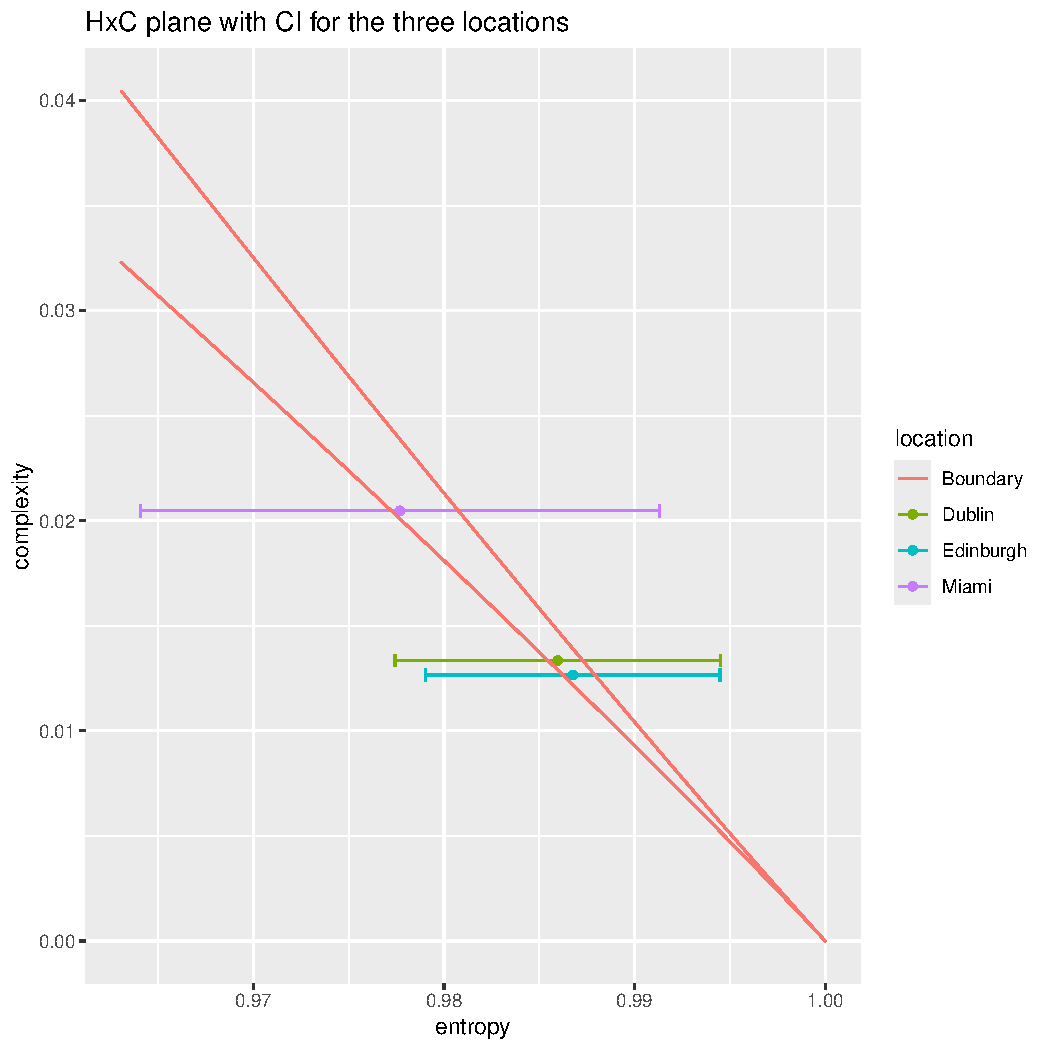
\includegraphics[width=\textwidth,keepaspectratio]{./Weather/confidenceIntervalPlot.pdf}
    \caption{HxC plane of locations with confidence interval}
\end{figure}

P values are calculated. 10 iterations are done on adding noise for breaking ties and compared with the p-value of the theoretical split. The theoretical p value is only larger than one iteration for Miami-Edinburgh, two for Miami-Dublin and four for Edinburgh-Dublin, which is OK. Ideally, it should be between iteration 5 and 6. Most importantly, it is the range of the iterations, which definitely confirms it is implemented so what correctly. 


Adding noise has a couple of problems in the sense that it is much more computer-intensive to calculate just 10 iterations compared with the theoretical value once.
'\begin{figure}
    \centering
    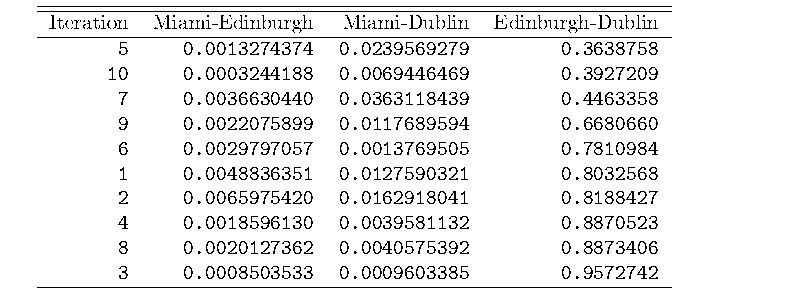
\includegraphics[width=\textwidth,keepaspectratio]{./Weather/pValuesTheoretical,10=Iterations,Sorted.pdf}
    \caption{Noise added, 10 iterations, sorted by column “Edinburgh-Dublin"}
\end{figure}

'\begin{figure}
    \centering
    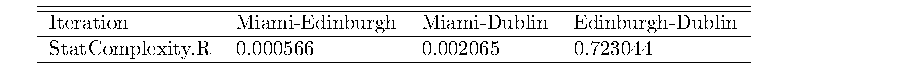
\includegraphics[width=\textwidth,keepaspectratio]{./Weather/pValuesTheoretical.pdf}
    \caption{p value, when using theoretical split}
\end{figure}


\chapter{Conclusion}
Metadata about the health of reproducibility in the scientific field of Ordinal Patterns were gathered and analysed. Clear traces and indicators of a reproducibility crisis equal to that seen in many other scientific fields. The other main finding of the paper is the analysis of tie-breaking. To ensure stable results, across current implementations of the libraries in the field, it is necessary to both add noise and remove Na values. The new method proposed that breaks ties evenly among possible patterns were analysed. It has the benefit of not needing to add noise, making it a deterministic method, whereas adding noise is a stochastic method. It performed very well for the entropy and should be considered when dealing with a dataset, with a large degree of ties. For the $p$-values, it was slightly less impressive, since its $p$-values were not as close to the median of the ten iterations. 
\chapter{Data Availability}
All data and code can be found in the GitHub: "https://github.com/polsemix101/Research-Project". The GitHub contains a detailed README, which explains the resporitary seetup

%%%%%%%%%%%%%%%%%%%%%%%%%%%%%%%%%%%%%%%%%%%%%%%%%%%%%%%

% and of course book style knows about backmatter
% \backmatter caused problems with appendices :-(
% and of course report style doesn't
%%%%%%%%%%%%%%%%%%%%%%%%%%%%%%%%%%%%%%%%%%%%%%%%%%%%%%%


\bibliographystyle{ieeetr}
\bibliographystyle{acm}
\bibliography{myrefs}


\end{document}
e